\documentclass[a4paper, 11pt, twocolumn]{article}

\usepackage[a4paper, total={6.24in, 8.5in}]{geometry}
\usepackage[utf8]{inputenc}
\usepackage{graphicx}
\usepackage{verbatim}
\usepackage{float}
\usepackage{array}
\usepackage{xfrac}
\usepackage{mathpazo}
\usepackage{amsmath}
\usepackage{bm}
\usepackage{multirow}
\usepackage{makecell}
\usepackage{multicol}
\usepackage{sectsty,textcase}
\usepackage{wrapfig,lipsum,booktabs}
\usepackage{enumitem}
\usepackage{hyperref}
\usepackage{makecell}
\usepackage{array}
\usepackage{layouts}

\bibliographystyle{plain}
\renewcommand{\thesection}{\arabic{section}}
\setlength{\columnsep}{15pt}
\newcommand{\myparagraph}[1]{\paragraph{#1}\mbox{}\\}

\title{FYS-STK3155/4155 Applied Data Analysis and Machine Learning - Project 3 }

\author{Lotsberg, Bernhard Nornes \\ Nguyen, Anh-Nguyet Lise \and
\url{https://github.com/liseanh/FYS-STK4155-project3}}
\date{November - December 2019}
\begin{document}
\twocolumn[
  \begin{@twocolumnfalse}
    \maketitle
    \begin{abstract}
		Whole page: \printinunitsof{in}\prntlen{\textwidth}
		Column: \printinunitsof{in}\prntlen{\columnwidth}
	\end{abstract}
  \end{@twocolumnfalse}
]


\section{Introduction}
In popular culture the neural network is probably the most well known form of
machine learning. In recent years many other statistical learning methods have
proven themselves as well however. In this project we compare the performance of
neural networks and gradient boosting in the case of binary classification.
In addition to these, we also use the much simpler k-nearest neighbours method
as a baseline for classification performance.



\section{Data}

The data set we will analyse in this project is the MAGIC Gamma Telescope data
set retrieved from the \href{https://archive.ics.uci.edu/ml/datasets/MAGIC+Gamma
+Telescope}{UCI Machine Learning Repository}, which was generated by a Monte
Carlo (MC) program described by D. Heck et. al. \cite{heck1998corsika} to
simulate high energy gamma particle registration in a Cherenkov gamma telescope.
The set consists of ten explanatory variables and a binary response variable
\texttt{class} which specifies whether the measured photons resulted from a gamma
particle (\texttt{class} = g) or a hadron (\texttt{class} = h). The entire data
set consists of 19020 instances with no missing values, with outcome distribution
as shown in Figure \ref{fig:Histogram}. The explanatory and response variables
are defined as the following by the UCI Machine Learning Repository
\cite{Dua:2019}:

\begin{enumerate}[leftmargin=5mm, itemsep=0pt,  parsep=1pt]
  \item \texttt{fLength}: continuous \# major axis of ellipse [mm]
  \item \texttt{fWidth}: continuous \# minor axis of ellipse [mm]
  \item \texttt{fSize}: continuous \# 10-log of sum of content of all pixels
        [in \#phot]
  \item \texttt{fConc}: continuous \# ratio of sum of two highest pixels over
        \texttt{fSize} [ratio]
  \item \texttt{fConc1}: continuous \# ratio of highest pixel over \texttt{fSize}
        [ratio]
  \item \texttt{fAsym}: continuous \# distance from highest pixel to center,
        projected onto major axis [mm]
  \item \texttt{fM3Long}: continuous \# 3rd root of third moment along major
        axis [mm]
  \item \texttt{fM3Trans}: continuous \# 3rd root of third moment along minor
        axis [mm]
  \item \texttt{fAlpha}: continuous \# angle of major axis with vector to origin
        [deg]
  \item \texttt{fDist}: continuous \# distance from origin to center of ellipse
        [mm]
  \item \texttt{class}: g, h \# gamma (signal), hadron (background)
\end{enumerate}


\begin{figure}
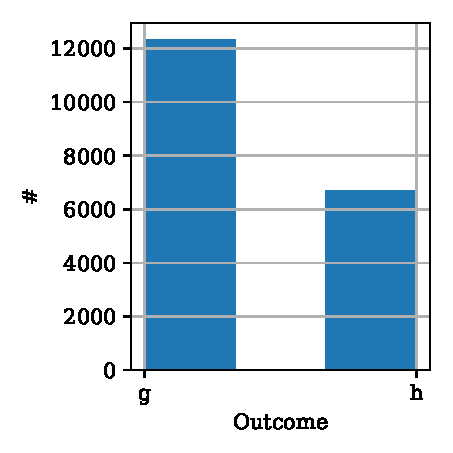
\includegraphics[scale=1]{{figures/histogram}.pdf}
\caption{Frequencies of the outcomes g and h in the data set. The numbers of
instances for the categories were 12332 and 6688 for g and h respectively.}
\label{fig:Histogram}
\end{figure}
m
\begin{figure*}
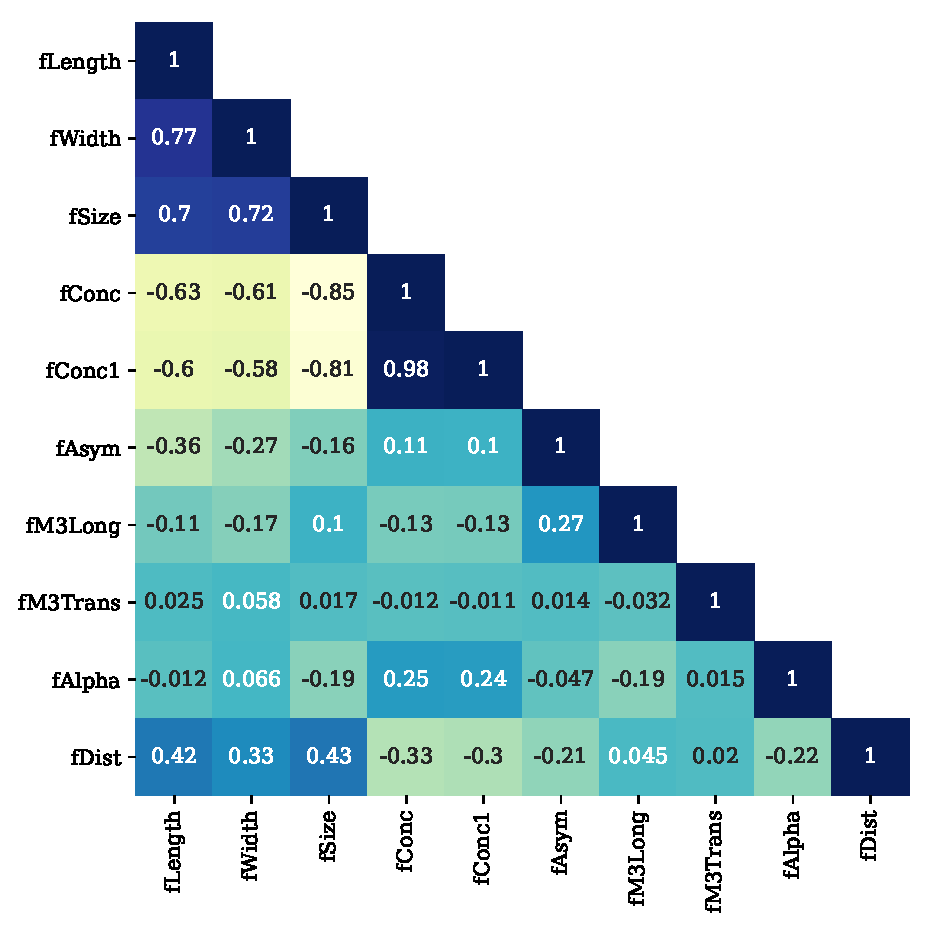
\includegraphics[scale=0.5]{{figures/correlation_matrix_train}.pdf}
\caption{Correlation matrix of the features in the train set. Upper triangle
excluded for readability.}
\label{fig:Correlation}
\end{figure*}
\section{Methods}

\subsection{$\pmb{k}$-Nearest Neighbour (kNN)}
The $k$-nearest neighbour method is a non-parametric method that consists of
using the $k$ observations in the training set in feature space closest to a point
$x$ to form a model $\hat{y}$. For regression and binary classification, the
method considers a point $x$ and the $k$ closest points $x_i$ in the
neighbourhood $N_k(x)$ defined by $k$, such that
\begin{equation} \label{eq:kNN}
\hat{y} = \frac{1}{k}\sum_{x_i\in N_k(x)} y_i,
\end{equation}
i.e. the model output is the average of the $k$ closest points to $x$.

As we are using this method for binary classification, we assign the classes such
that
\begin{equation}
\hat{Y}=
\begin{cases}
      \text{g if }  \hat{y}\leq 0.5\\
      \text{h if } \hat{y} > 0.5
\end{cases} \cite{hastie}.
\end{equation}

Alternatively, the observation can be assigned according to the majority class of
its neighbours, such that the observation is classified as the most common class
in its neighbourhood. This is the method used for multiclass classification.

To implement kNN and the hyperparameter optimisation in this project we use the
\href{https://scikit-learn.org/stable}{Scikit-Learn}
library.

\subsubsection{Hyperparameter tuning}
The kNN method is a simple approach that only requires tuning of a single
hyperparameter $k$. Using $k=1$ results in a highly complex model with high
variance, while using $k=N$, where $N$ is the total number of samples in the
training set, results in a simple, highly biased model. To find the optimal value
for $k$ in our case, we use 5-fold cross-validation on the training set, keeping
1/3rd of the total data as test set.


\subsection{Multilayer Perceptron (MLP)}
A multilayer perceptron (MLP) is a feed-forward neural network. It contains an
input layer, one or more hidden layers, with tunable number of nodes and layers,
and a final output layer. The information flows only in one direction from the
input layer to the output layer. The input and output values of the nodes are
determined by an activation function, in addition to the weights and biases of
the nodes. For a more extensive explanation of how the different components of
the MLP works, please refer to our previous work, \textit{Project 2: Regression
and Classification} \cite{project2}.

We have chosen to use the Rectified Linear Unit (ReLU) function as our
activitation function $f(z)$ between the layers, which is given by
\begin{equation}
      f(z) = \max (0,\ z),
\end{equation}
and its gradient by
\begin{equation}
      f'(z) =
      \begin{cases}
            0, &  z<0\\
            1, &  z>0
      \end{cases}.
\end{equation}
For the activation function of the final output layer, we use the softmax
function to achieve the categorical outcomes,
\begin{equation}
      f(z_i)=\frac{\exp(z_i)}{\sum \exp(z_j)}
\end{equation}

For this project we will be using the \href{https://www.tensorflow.org/}
{TensorFlow} library to implement the MLP with the addition of the
\href{https://scikit-optimize.github.io/}{Scikit-Optimize} library to optimise
the hyperparameters.

\subsubsection{Hyperparameter tuning}
In this project we choose to limit ourselves to two hidden layers for 
computational reasons, and tune the amount of nodes in both of those layers.

To counteract the high variance of the model, we introduce regularisation using 
dropout. Dropout is tuned for eachlayer, and is the chance of any node in the 
given layer to be ignored at an iteration in training. This reduces variance by 
forcing the other nodes to be able to work more independently from each other, 
lessening the chance for overfitting.

We also tune the batch size. This leaves us with five hyperparameters to tune. A 
grid search would be too expensive to perform, so instead we perform a random
search. Ideally we would employ cross validation on the train set evaluate the 
candidate hyperparameters, but for computational reasons we have decided to 
instead set aside 10\% of the training set for validation. After finding the 
tuning parameters that maximise F$_1$ on the validation set, we use these 
parameters to fit the model on the entire training data including the validation 
data. This is known as a refit. 


\subsection{Gradient Boosting and Extreme Gradient Boosting (XGB)}
Boosting is a learning technique based on the idea of combining several weak
learners $b_m$ into a final strong learner $f_{m_\text{stop}}$, where each
$f_m$ is improved from the previous iteration $f_{m-1}$ through the step $h_m$,
\begin{equation}
      f_{m_\text{stop}} = \sum_{m=0}^{m_\text{stop}} h_m.
\end{equation}

Gradient boosting is one such method. We consider a loss function $L(y, f(x))$,
which is minimised by calculating the negative gradient of the loss
function to obtain the minimisation direction. To prevent overfitting, the
boosting step size, also referred to as learning rate, $\nu \in (0,1)$ is 
introduced as a tuning parameter, with smaller values of $\nu$ resulting in 
larger shrinkage, 
\begin{equation}
f_m(x)=f_{m-1}(x) + \nu h_m .
\end{equation}
The gradient boosting algorithm goes as follows: \cite{RiccardoGB}
\begin{enumerate}[leftmargin=5mm, itemsep=0pt,  parsep=1pt]
\item Initialize the estimate $f_0(x)$
\item for $m= 1,\ ,\dots,\ m_\text{stop}$:
      \begin{enumerate}[leftmargin=5mm, itemsep=0pt,  parsep=1pt]
            \item Compute negative gradient vector
            \begin{equation*}
                  u_m = -\frac{\partial L(y,\ f(x))}{\partial f(x)} \bigg\vert
                  _{f(x)=\hat{f}_{m-1}(x)}
            \end{equation*}
            \item Fit the base learner to the negative gradient vector,
            $b_m(u_m, x)$
            \item Update the estimate
            \begin{equation*}
                  f_m(x) = f_{m-1}(x) + \nu b_m (u_m, x)
            \end{equation*}
      \end{enumerate}
\item Compute final estimate,
      \begin{equation*}
            \hat{f}_{m_\text{stop}} (x) =
            \sum _{m=0}^{m_\text{stop}-1}\nu b_m(u_m, x)
      \end{equation*}
\end{enumerate}

For this project, we have chosen to boost decision trees using a variant of
gradient boosting called extreme gradient boosting (XGB).


\subsubsection{Hyperparameter tuning}
The XGBoost package has many hyperparameters added on top of the ordinary 
gradient boosting algorithm. 

The learning rate $\nu$

As with the neural network model, we also do not use cross validation here. We 
use the same train-validation split as for the neural network. We also employ
a randomised search instead of a grid search.

\subsection{Model evaluation}
For classification problems, one can visualise the performance of a model using the so called confusion matrix. In our case it is defined as.
\begin{align}
\bm{A}&=\begin{pmatrix}
\sum (\hat{y}=g, y=g) & \sum(\hat{y}=h, y=g) \\
\sum(\hat{y}=g, y=h) & \sum(\hat{y}=h, y=h)
\end{pmatrix}\nonumber \\
&=\begin{pmatrix}
g_g & g_h \\
h_g & h_h
\end{pmatrix}.
\label{eq:Confusion}
\end{align}
A perfect model would then only have elements on the diagonal.

A common way to evaluate classification models is the F$_1$-score. This is a 
metric quantifying the amount of diagonal and off-diagonal elements of the 
confusion matrix and is defined as 
\begin{equation}
\text{F}_1=\frac{2 g_g}{2g_g + g_h + h_g}
\label{eq:F1}
\end{equation} 
The F$_1$ score can vary between 0 and 1, 1 representing a perfect fit with 
no off-diagonal elements. To us the best performing model is the model which 
maximises $F_1$ and minimises $g_h$ on the test set, as false negatives are 
worse than false positives in this case because they lead to loss of important 
data.

\section{Results}

Figure \ref{fig:Correlation} shows the correlation of the features in the
training set. Some of the features are highly correlated to each other.

Table \ref{tab:F1} shows the train and test F$_1$
scores for the three models employed in this project.
XGBoost seems to outperform the neural network by a
small margin for this split of the data. Both the
neural network and XGBoost clearly outperform kNN.
This is also evident in the confusion matrices shown
in Figure \ref{fig:kNN}, \ref{fig:NN_confusion} and
\ref{fig:XGB_confusion}. Both the number of false
positives and false negatives are lowest for XGBoost.

For kNN, the tuning parameter $k$ was found to be best
at $k=5$. This is also evident in Figure
\ref{fig:kNN}. The estimated hyperparameters for MLP and
XGBoost are stated in Table \ref{tab:Tune_NN} and
\ref{tab:Tune_XGB}.


\begin{table}[H]
\caption{Estimated optimal hyperparameters found using randomised search for the 
multilayer perceptron model.}
\label{tab:Tune_NN}
\resizebox{\columnwidth}{!}{
  \begin{tabular}{|l|l|} \hline 
      \textbf{Hyperparameter} & \textbf{Optimal value} \hspace{2pt} \\ \hline
      Batch size              & 109              \\ \hline
      Epochs                  & 55               \\ \hline
      Dropout, first layer    & 0.13             \\ \hline 
      Dropout, second layer   & 0.095            \\ \hline 
      Nodes, first layer      & 17               \\ \hline 
      Nodes, second layer     & 4                \\ \hline 
  \end{tabular}
}
\end{table}


\begin{table}[H]
\caption{Estimated optimal hyperparameters found using randomised search for the 
extreme gradient boosted tree model.}
\label{tab:Tune_XGB}
\resizebox{\columnwidth}{!}{
  \begin{tabular}{|l|l|} \hline
      \textbf{Hyperparameter} & \textbf{Optimal value} \hspace{2pt} \\ \hline
      Learning rate           & 0.048     \\ \hline 
      Epochs                  & 125       \\ \hline 
      Maximum  tree depth     & 9         \\ \hline 
      L1 shrinkage parameter  & 0.0074    \\ \hline 
      L2 shrinkage parameter  & 0.0035    \\ \hline 
      Minimum child weight    & 3         \\ \hline 
  \end{tabular}
}
\end{table}
      
      

\begin{table}[H]
\caption{F$_1$ score for the training and test set for our k-nearest neighbour 
(kNN), multilayer perceptron (MLP) and extreme gradient boost (XGB) models .}
\label{tab:F1}
\resizebox{\columnwidth}{!}{
\begin{tabular}{|l|l|l|l|}
\hline
\textbf{F$_1$ score}  & \textbf{kNN} \hspace{10pt} 
& \textbf{MLP} \hspace{10pt} & \textbf{XGB}  \hspace{10pt}\\ \hline
Training set & $0.88$ & $0.87$ & $0.95$ \\ \hline
Test set     & $0.83$ & $0.87$ & $0.88$ \\ \hline
\end{tabular}
}
\end{table}

\begin{figure*}
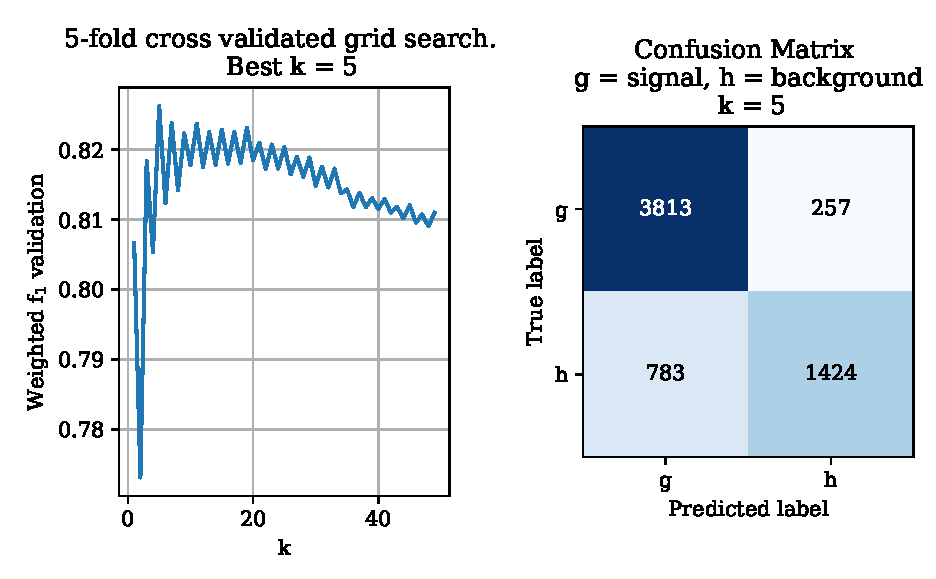
\includegraphics[scale=1]{{figures/kNN_cv_results}.pdf}
\caption{Results from tuned kNN using cross validation. The confusion matrix was
found using the test set.}
\label{fig:kNN}
\end{figure*}

\begin{figure}
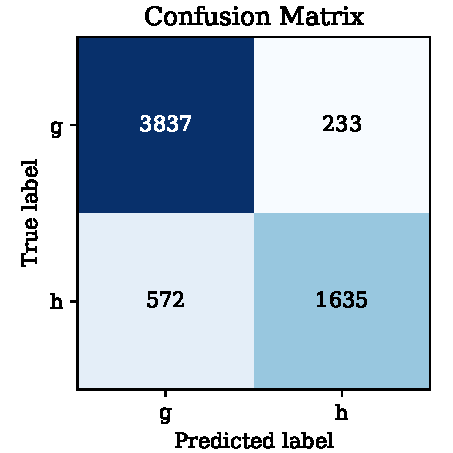
\includegraphics[scale=1]{{figures/nn_confusion_matrix}.pdf}
\caption{Confusion matrix of the neural network model applied to the test set.}
\label{fig:NN_confusion}
\end{figure}

\begin{figure}
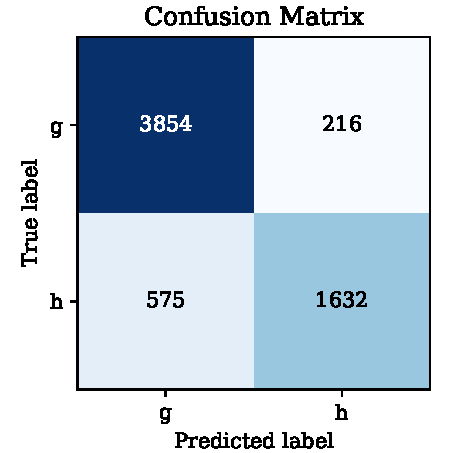
\includegraphics[scale=1]{{figures/xgboost_confusion_matrix}.pdf}
\caption{Confusion matrix of the gradient boosted model applied to the test set.}
\label{fig:XGB_confusion}
\end{figure}

\section{Discussion}

\section{Conclusion}


\section*{Acknowledgements}
We want to thank the University of California, Irving for providing us with the
data used in this project.


%\bibliographystyle{iEEEtran}
\bibliography{bibliography}



\end{document}
